We wish to model the effects of the cellular retinoic acid binding proteins
(crabps) and Cyp26a1 on the noise of the RA gradiant in zebrafish hindbrain
development.
\begin{tabular}{ c c }
{\parbox{.4\textwidth}{
\begin{itemize}
\item Assume the regulation of RA is Michaelis-Menton.
\item Let $\eta$, the basal rate of RA degradation, be a "small but not insignificant" constant.
\item Let $[Crabp]$ effect the binding of RA to RA-R and of Cyp26a1 to RA linearly.
\item Let $[Cyp]_{max}$ be the maximum upreglated Cyp26 due to RA-R. 
\end{itemize}}}
& 
\raisebox{-.5\totalheight}{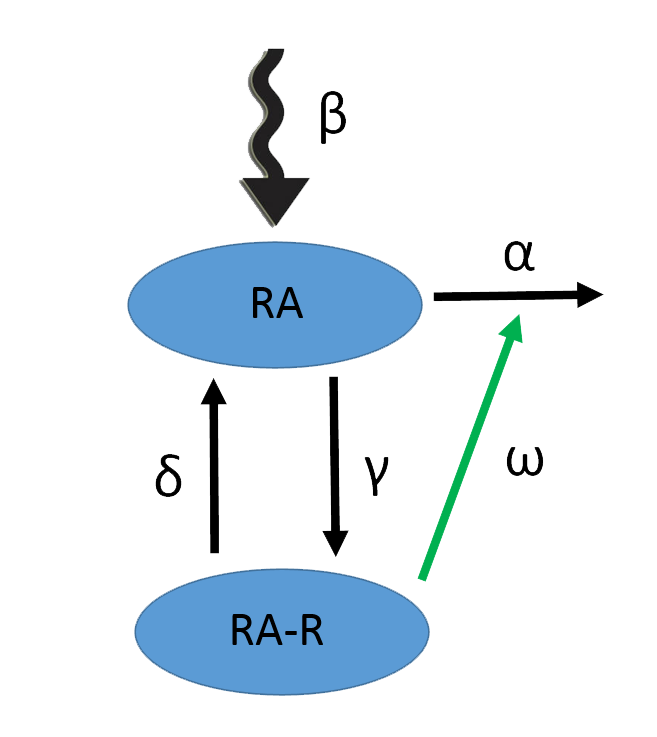
\includegraphics[scale=0.34]{figures/RAPNetwork.PNG}}
\end{tabular}

\footnotesize
\begin{eqnarray*} 
d[RA] & = & [\beta-\left(\frac{\alpha_{0}[Cyp]_{max}[RA-R]}{\omega_{0}/[Crabp]+\omega_{1}+[RA-R]}+\gamma_{0}[Crabp]+\gamma_{b}+\eta\right)[RA] \\
& & + \delta[RA-R] ]dt+\sigma dW_{t}\\
d[RA-R] & = & \left((|\gamma_{0}[Crabp]+\gamma_{b})[RA]-\delta[RA-R]\right)dt\\
d[Crabp] & = & 0
\end{eqnarray*}


